\section{Environnement Logiciel}

\subsection{Librairies et frameworks utilis�s}
\begin{frame}{Environnement Logiciel}
    \begin{block}{Elasticearch}
        \begin{itemize}
            \item Moteur d'indexation
            \item Puissant et distribu� (recherche en temps r�el)
            \item Int�gre deux moteurs de recherche : document et index
        \end{itemize}

    \end{block}
    
    \begin{block}{SableCC}
        \begin{itemize}
        	\item Analyse LALR (Look Ahead Lef Recursive)
            \item G�n�rateur de compilateur
            \item Parseur contruit automatiquement l'AST
            \item N{\oe}uds de l'AST strictement typ�s
            \item N{\oe}uds parcourus par un visiteur
            \item Visiteur utilise le Pattern visitor
        \end{itemize}

    \end{block}

\end{frame}

%

\subsection{D�marche de d�veloppement}
\begin{frame}{JUnit}
    \centering
    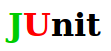
\includegraphics[scale=0.7]{./images/junit_logo.png}

    \begin{block}{}
        \begin{itemize}
            \item Test Driven Development
            \item Ecriture de tests unitaires
            \item Description des exigences du code
        \end{itemize}

    \end{block}

\end{frame}